\subsection{Connections between the AE modules}
Figure~\ref{fig:ae_modules} expands the AE heads and their supervision.
The reference dense encoder begins with a factor-four patch stem, followed
by stage-matched residual convolutions and downsampling to a $10^3$ grid.
The code has 64 channels. The implementation also retains an occupied-voxel
sparse encoder for future efficiency experiments; it densifies its bottleneck
for the same decoder and heads. It is not used by the reported checkpoints.

The dense decoder applies five residual/convolutional upsampling stages,
with spatial sizes $10,20,40,80,160,320$ and channels
$64,48,32,24,16,8$. Final $1\times1\times1$ heads predict occupancy logits
and unsigned distance. Four intermediate occupancy heads attach at spatial
sizes $20,40,80,160$. The query head instead samples the noisy code at a
query coordinate, concatenates normalized coordinates, and applies a
width-128 MLP. There are no encoder--decoder skip connections.

\begin{figure*}[t]
 \centering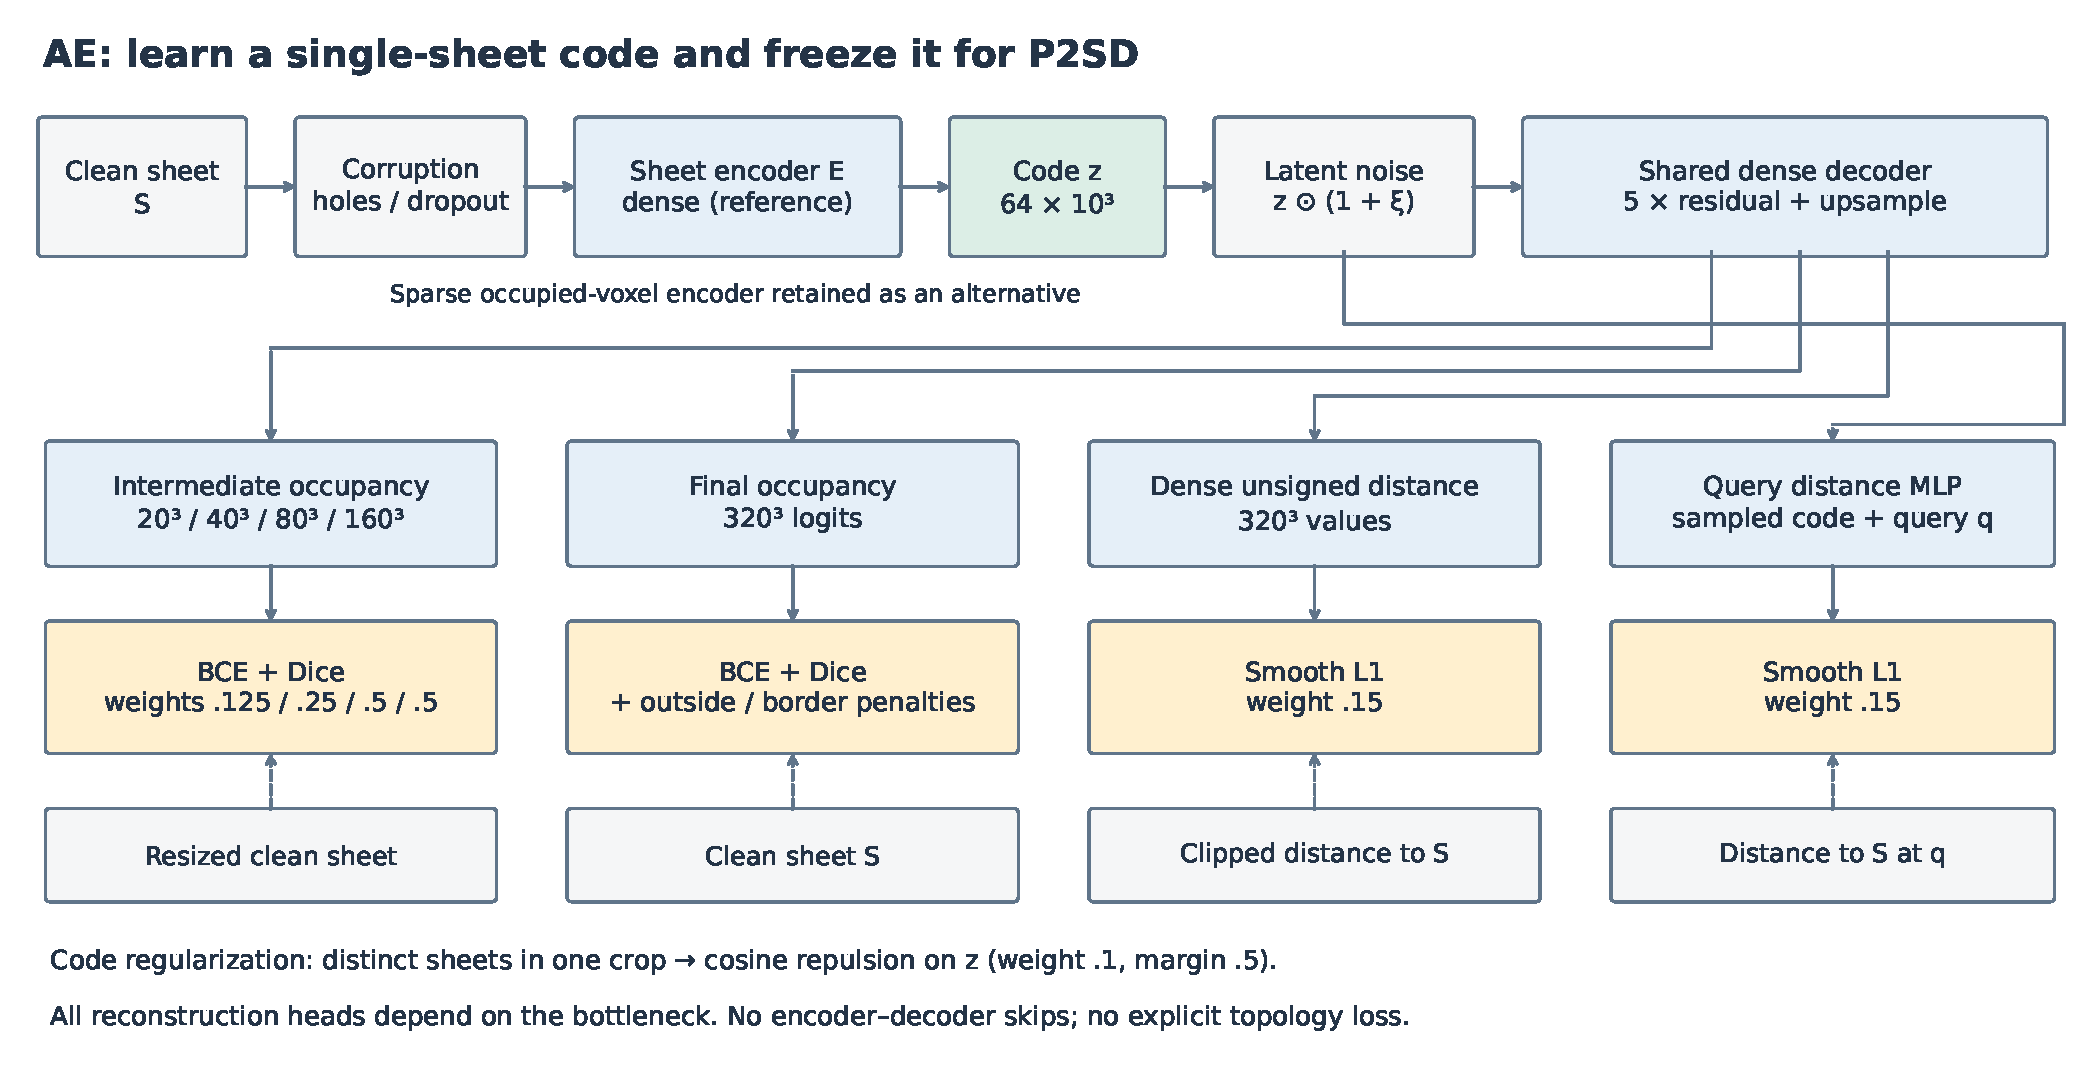
\includegraphics[width=\textwidth]{figures/ae_modules.pdf}
 \caption{\textbf{AE modules and supervision.} Decoder occupancy and distance
 heads share dense features; query distance is predicted directly from the
 noisy latent code. Each loss is paired with its target. Intermediate heads
 attach at successive decoder stages. Code repulsion acts on distinct-sheet
 codes before latent noise. The sparse encoder remains an optional alternative.}
 \label{fig:ae_modules}
\end{figure*}

\subsection{Connections between the P2SD modules}
Figure~\ref{fig:p2sd_modules} separates shared image computation from
prompt-dependent computation. The image encoder reduces CT to a
$512\times10^3$ feature grid. A $1\times1\times1$ projection and four
self-attention blocks form the image context $F$: 1,000 tokens of width 512.
Three-dimensional per-axis rotary coordinates supply position information.

For each prompt coordinate $p_k$, prompt composition concatenates its
eight-band Fourier encoding, the trilinearly sampled context $F(p_k)$,
and the positive-label scalar. A two-layer MLP produces one width-512 token
per point. The reference retains all $K$ prompt tokens. The prompt modulator
prefixes them to the context tokens, aligns their coordinate frames for
rotary attention, and applies one attention block. Prompt-prefix outputs
are discarded; the remaining 1,000 conditioned grid tokens enter the refiner.

The refiner contains four self-attention blocks with eight heads and SwiGLU
MLPs. Linear projections supply intermediate code estimates; a separate
LayerNorm and linear projection supply the final normalized 64-channel code.
The loss distinguishes these auxiliary projections from the final head, as
specified in Eq.~\ref{eq:p2sdloss}. Channel statistics come from training-sheet
AE codes. Inference reverses this normalization before the frozen AE decoder.

The binary branch receives the \emph{unprompted} image context, applies its
own four attention blocks, and upsamples with residual/convolutional stages
of channels $512,256,128,64,32,16$. A final $1\times1\times1$ head produces
union logits. It has no encoder--decoder skip connections; residual
connections inside individual blocks are distinct. Its loss updates the
shared image encoder and image-context blocks. In the new training recipe,
refinement sees the complete $10^3$ context and decoding builds the full
$160^3$ intermediate feature grid. We crop $80^3$ features there and apply
the final $\times2$ upsampling, residual block and occupancy head to obtain
$160^3$ output supervision. Earlier stages retain full-volume context at
increased activation-memory cost. This is the retained \texttt{second\_last}
crop mode, also used by 0076. The scored 0058 checkpoint instead used an
earlier $5^3$ context crop; its measurements are unchanged.

\begin{figure*}[t]
 \centering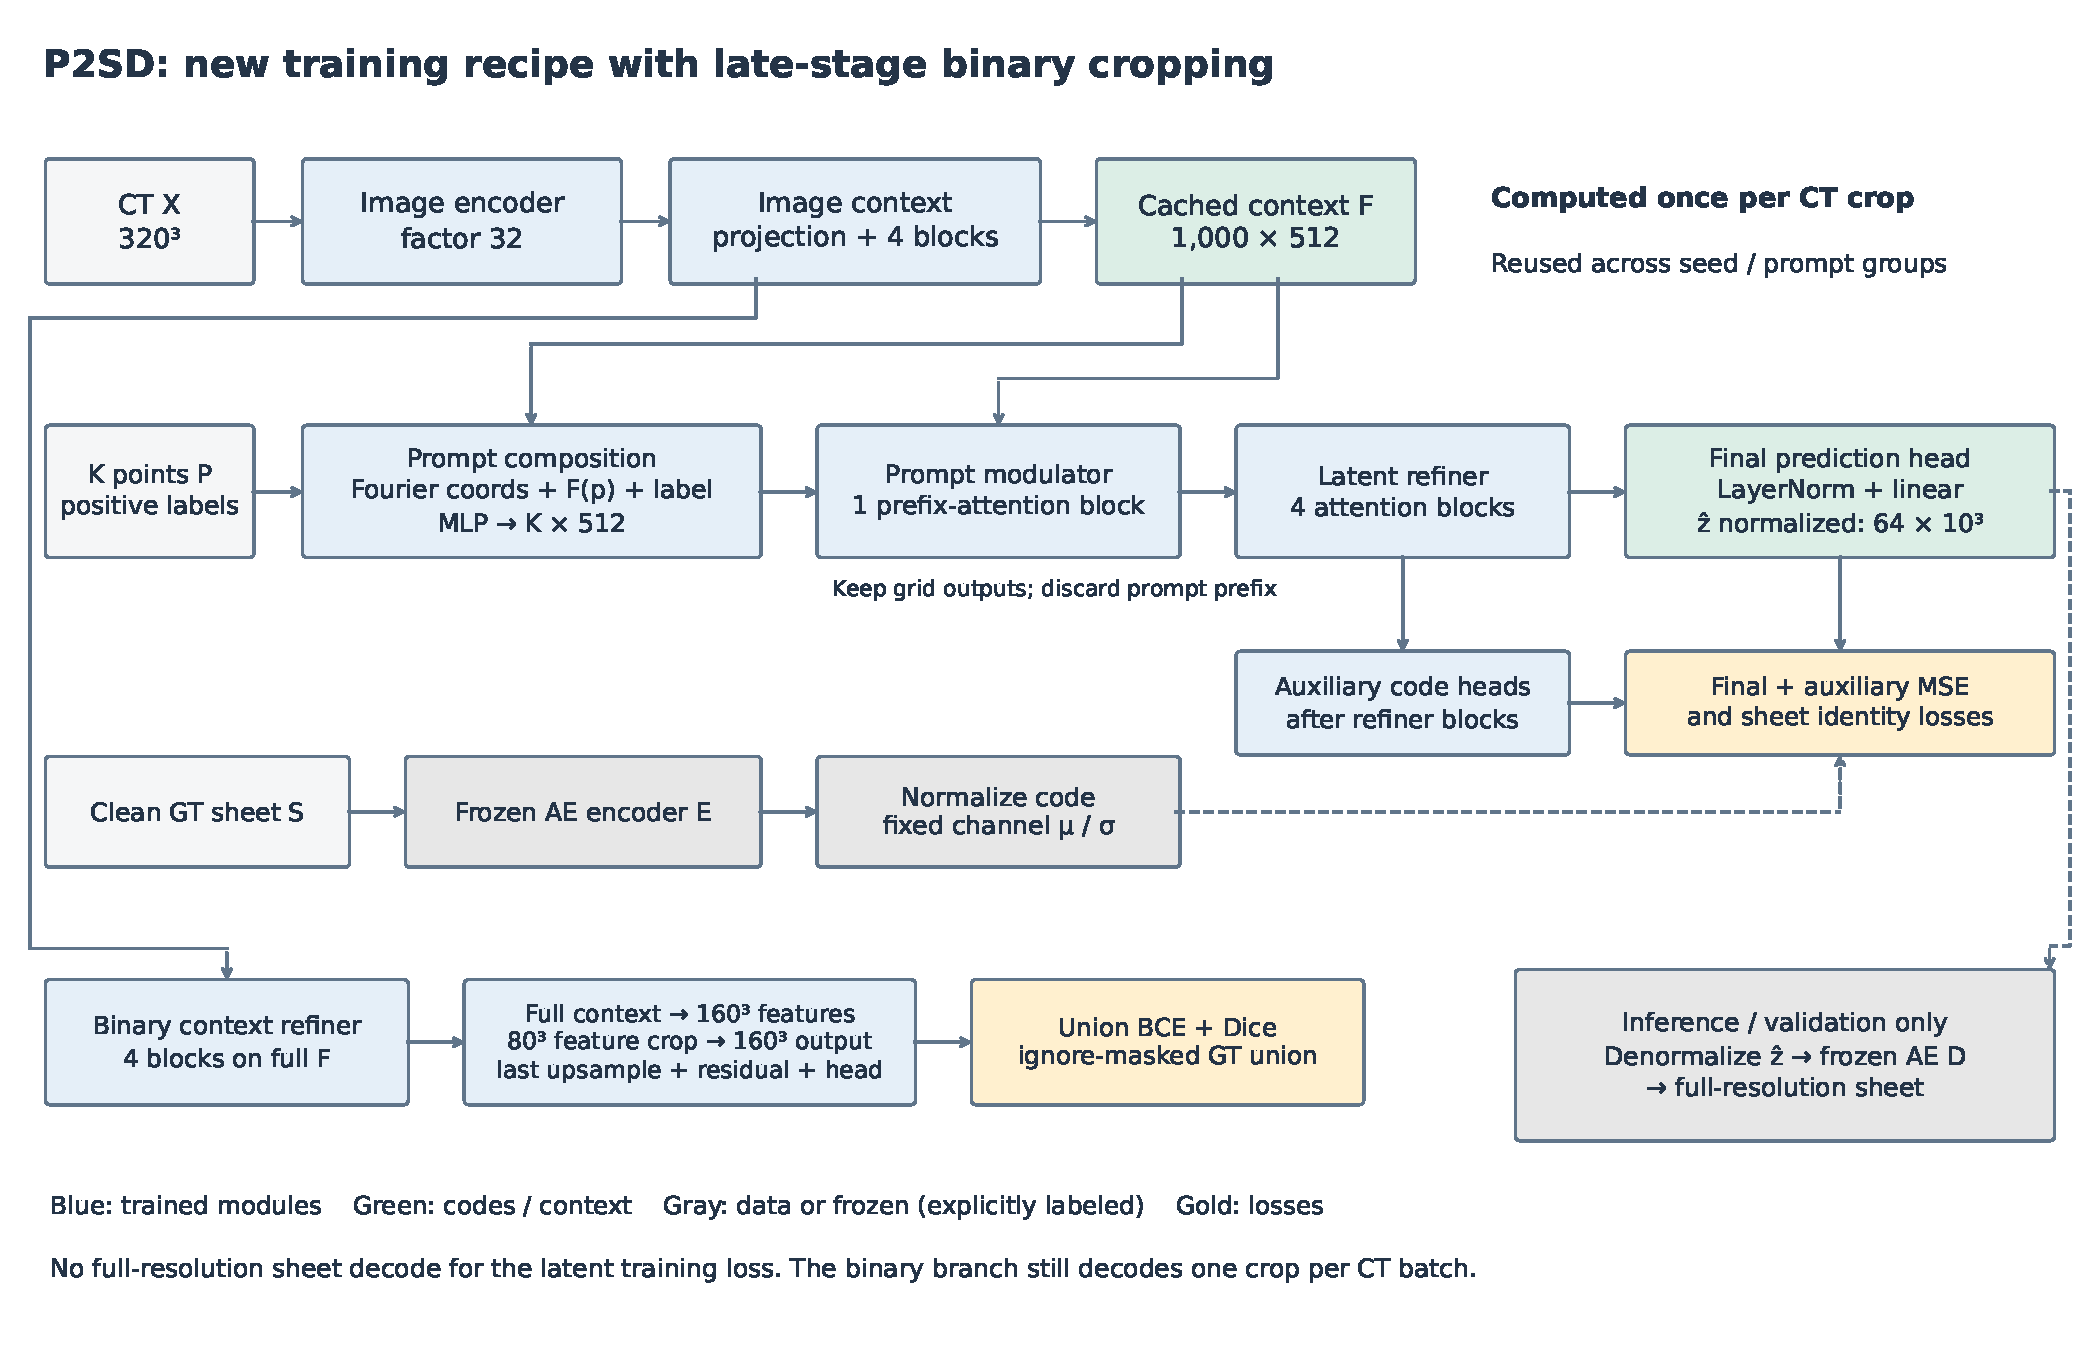
\includegraphics[width=\textwidth]{figures/p2sd_training_recipe.pdf}
 \caption{\textbf{P2SD modules in the new training recipe.} Shared CT encoding
 and context feed prompt composition, modulation and refinement. Code heads
 learn from the frozen AE. The binary branch decodes full context to $160^3$
 features before cropping for its final upsampling; at inference it decodes
 the full union for seed proposal. The sheet decoder is used only when masks
 are needed under the main latent objective. Optional query losses are
 described separately; the scored 0058 checkpoint used earlier cropping.}
 \label{fig:p2sd_modules}
\end{figure*}

\subsection{Efficiency of compact latent prediction}
For a $320^3$ crop, prompt conditioning and code prediction operate on only
$10^3=1{,}000$ spatial sites, compared with $32{,}768{,}000$ output voxels.
Including its 64 channels, a sheet code has 64,000 scalars, 512 times fewer
than one full-resolution scalar mask. At BF16, these tensors occupy
0.122 MiB and 62.5 MiB, respectively; the shared $512\times10^3$ context
occupies 0.977 MiB. These are tensor-size comparisons, not measured speedups
or total training-memory estimates. Attention still incurs token-pair work.

Let $N$ be the number of foreground seeds, $G$ the number of additional
multi-point prompt groups used for cluster consistency, and $K$ the number
of sheet hypotheses that are densely decoded. Let $C_{\rm img}$ denote
shared CT encoding/context cost, $C_{\rm code}$ the cost per prompt group,
$C_{\rm cluster}$ clustering cost, $C_B$ the binary branch's refinement and
union decoding cost, and $C_D$ one AE decoding cost. With the co-trained
proposal head, automatic inference has approximate cost
\begin{equation}
 C_{\rm img}+C_B+(N+G)C_{\rm code}+C_{\rm cluster}+K C_D.
\end{equation}
This avoids paying a full upsampling cost for each of the $N$ seed codes
before clustering. Retained sheets still require dense decoding, output
storage and cleanup. The co-trained proposal head reuses the cached image
context and incurs one full-resolution union decode. The historical benchmark
instead uses a separate proposer with its own CT encoder, so its cost includes
an additional encoding. No binary training crop is applied at inference.

During P2SD training, the frozen teacher encoder produces sheet targets, but
the active latent objective does not require AE decoding. The auxiliary
binary branch still decodes a crop once per CT batch, and validation decodes
full sheet masks. We therefore claim an architectural advantage in repeated
prompt processing, rather than an unmeasured end-to-end runtime advantage.
